\chapter{Antecedentes}
\label{chp:antecedentes}

\section{Introducción}
En este capítulo se abordan las generalidades sobre el origen del agua producida y los conceptos como la canalización y conificación de agua en yacimientos naturalmente fracturados. Luego se presenta una breve recopilación de la metodología que existe para su control y remediación. Adicionalmente, se introduce al espacio de los sistemas multifásicos dispersados con la idea de poner en contexto su aplicación en procesos de producción en pozos petrolíferos. Finalmente, se revisan algunos conceptos importantes relativos a las propiedades de la matriz poroso y a la interacción con los fluidos del yacimiento.

\section{Origen del agua producida}
Independientemente del tipo de fluido que se produce de un yacimiento, el agua comúnmente referida como \emph{intersticial} ó \emph{congénita} está presente en el yacimiento dentro de los poros que son suficientemente pequeños para retenerla mediante fuerzas capilares.

Dado que las rocas de un yacimiento son en su mayoría de origen sedimentario, se sabe que el agua se encontraba presente junto con el sedimento previo a los procesos diagenéticos, y por ello fue atrapada en los poros de la roca. Esta agua también puede moverse o pudo haber migrado debido a las presión hidráulica inducida por los procesos geológicos que también forman los yacimientos (\cite{Water1}). En los yacimientos de hidrocarburos siempre existirá una parte de esta agua que no fue desplazada hacia un horizonte acuífero por la migración del petróleo (\cite{StandardHandbook}).

Se sabe que la cantidad de agua intersticial suele ser inversamente proporcional a la permeabilidad del depósito. El contenido de agua congénita en los depósitos productores de hidrocarburos varia a menudo del $10\%$ al $40\%$.

Casi todos los yacimientos productores de hidrocarburos están rodeados por formaciones saturadas de agua llamadas acuíferos Estos acuíferos pueden ser sustancialmente más grandes que los depósitos de aceite y/o gas adyacentes de manera que parecieran de tamaño infinito, o pueden ser tan pequeños que sus efectos sean insignificantes sobre el comportamiento del yacimiento (\cite{Tarek}).

A medida que los fluidos del yacimiento son producidos y la presión del yacimiento declina, se crea un diferencial de presión del acuífero asociado hacia el yacimiento. Siguiendo las leyes básicas del flujo de fluidos en medios porosos, el acuífero reacciona invadiendo el yacimiento a través del contacto agua aceite. Este proceso resulta conveniente para la producción de aceite y gas, dado que cada barril de fluido producido será reemplazado por un barril de agua lo que mitiga la despresurización prematura del yacimiento e incrementa el factor de recuperación.

Esta invasión depende tanto de la permeabilidad del acuífero, que gobierna el diferencial de presión necesario para que la entrada de agua ocurra, así como del tamaño del acuífero en relación con el del yacimiento.

El agua producida en un pozo también puede provenir de pozos inyectores vecinos, ya que la inyección de agua es una de las operaciones mas comunes de la  recuperación secundaria, esta agua inyectada tiene la función de reemplazar dentro de la roca los fluidos que son producidos, de manera que hace mas eficiente el barrido del aceite y gas hacia los pozos.

\section{Problemática}
Se estima que a nivel mundial por cada barril de de petróleo producido se produce con el tres barriles de agua (\cite{Seright2001}). El costo anual por el manejo de agua producido le cuesta a la industria petrolera alrededor de $50$ mil millones de dolares (\cite{Hill2012}), este costo incluye tanto la descarga, el transporte reinyección y tratamiento para la correcta disposición del agua de producción. Este costo sin embargo no captura el costo indirecto asociado con la perdida o retraso de la producción debido a :

\begin{itemize}
    \item Pérdida de producción por aumento de la columna hidrostática.
    \item Flujo preferencial de agua sobre el aceite.
    \item Falta de capacidad en instalaciones para el manejo de agua.
    \item Migración de finos.
    \item Incidentes mecánicos asociados con corrosión y depósitos inorgánicos.
    \item Cierre y abandono de intervalos y pozos.
\end{itemize}

Los problemas asociados con la producción excesiva de agua se han clasificado en al menos $10$ categorías generales (\cite{Bailey2000}).



\subsection{Fugas}
Incluidas las fugas por detrás de la tubería de revestimiento empacadores y tubería de producción, permiten la entrada de agua de zonas no productoras de hidrocarburos hacia la corriente de producción (\autoref{fig:agua1}). En este caso la detección del problema y la aplicación de una solución dependen en gran medida de la configuración y estado mecánico del pozo. Los registros de producción como los de temperatura, densidad y los giroscópicos normalmente son suficientes para el diagnostico de este problema.

\begin{figure}\centering
    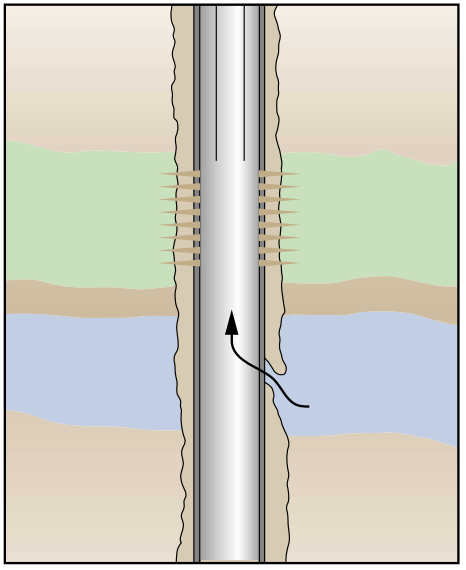
\includegraphics[width=0.5\textwidth]{Graphics/agua1.png}
    \caption[Fugas dentro del pozo]{Ejemplo de una fuga a través del revestimiento, \emph{tubing} o empacador. \emph{Adaptado de (\cite{Bailey2000})}.}
    \label{fig:agua1}
\end{figure}

\subsection{Canalización detrás del revestimiento}
Una cementación fallida puede conectar zonas acuíferas con intervalos productores (\autoref{fig:agua2}). Estos canales de flujo permiten que el agua fluya detrás de la tubería de revestimiento por el espacio anular. Otra posible causa de la canalización, puede ocurrir cuando la producción de arena  genera el derrumbamiento del pozo y crea un área vacía detrás del revestimiento propiciando el flujo de agua).

\begin{figure}\centering
    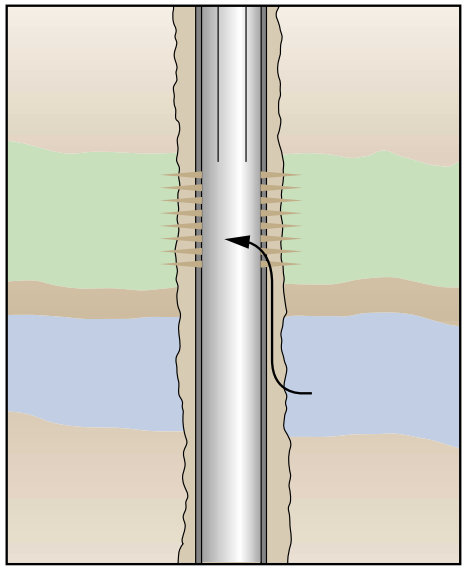
\includegraphics[width=0.5\textwidth]{Graphics/agua2.png}
    \caption[Canalización detras del revestimiento]{Ejemplo de canalización detrás del revestimiento. \emph{Adaptado de (\cite{Bailey2000})}.}
    \label{fig:agua2}
\end{figure}

\subsection{Contacto agua-aceite móvil}
Durante la producción en un yacimiento con empuje de acuífero asociado, el contacto agua aceite avanzando hacia la zona perforada puede resultar en una producción de agua económicamente insostenible. Este fenómeno puede ocurre en formaciones con permeabilidades verticales tan bajas como $K_{v}<0.01[mD]$, dado que el movimiento del contacto ocurre de manera lenta (\autoref{fig:agua3}).

\begin{figure}\centering
    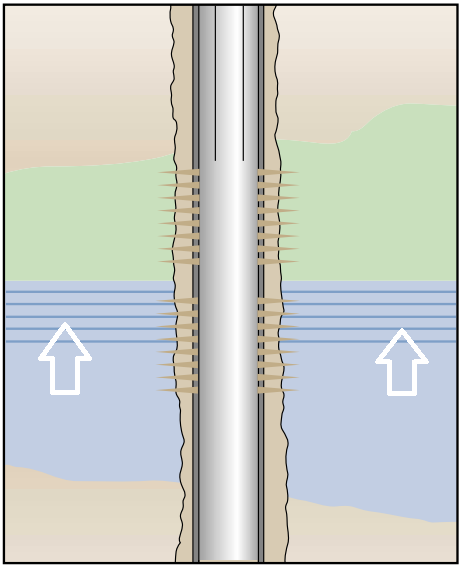
\includegraphics[width=0.45\textwidth]{Graphics/agua3.png}
    \caption[Movimiento del contacto agua aceite]{Movimiento del contacto agua aceite. \emph{Adaptado de (\cite{Bailey2000})}.}
    \label{fig:agua3}
\end{figure}


\subsection{Capa de riego sin flujo transversal}
Un problema común durante la producción simultanea de intervalos ocurre cuando un estrato o zona de alta permeabilidad que posee una barrera de flujo (como una capa de lutita) conduce el agua directamente hacia el pozo productor (\autoref{fig:agua4}). La fuente del agua puede ser un acuífero activo o un pozo inyector. Como no existe el flujo transversal este problema puede ser fácilmente atacado mediante agentes gelantes o selladores mecánicos dentro del pozo.

\begin{figure}\centering
    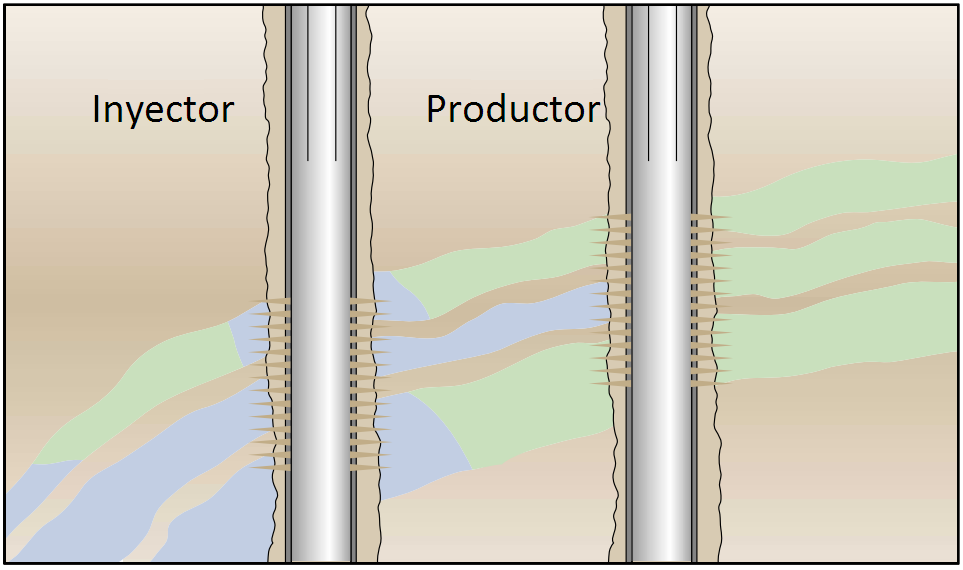
\includegraphics[width=0.8\textwidth]{Graphics/agua4.png}
    \caption[Capa de riego sin flujo transversal]{Capa de riego sin flujo transversal entre intervalos. \emph{Adaptado de (\cite{Bailey2000})}.}
    \label{fig:agua4}
\end{figure}


%\subsection{Digitalización}
\subsection{Fallas y fracturas entre inyector y productor}
En formaciones naturalmente fracturadas, la inyección de agua puede rápidamente avanzar hasta los pozos productores ()\autoref{fig:agua5}. Esto es común cuando el sistema de fracturas es extenso o fisurado y puede ser confirmado mediante el análisis de pruebas de presión y el uso de trazadores. Los registros de trazadores pueden también estimar el volumen de fracturas para diseñar el método de remediación. El uso de geles ha demostrado ser una opción viable para mitigar la producción excesiva de agua.

\begin{figure}\centering
    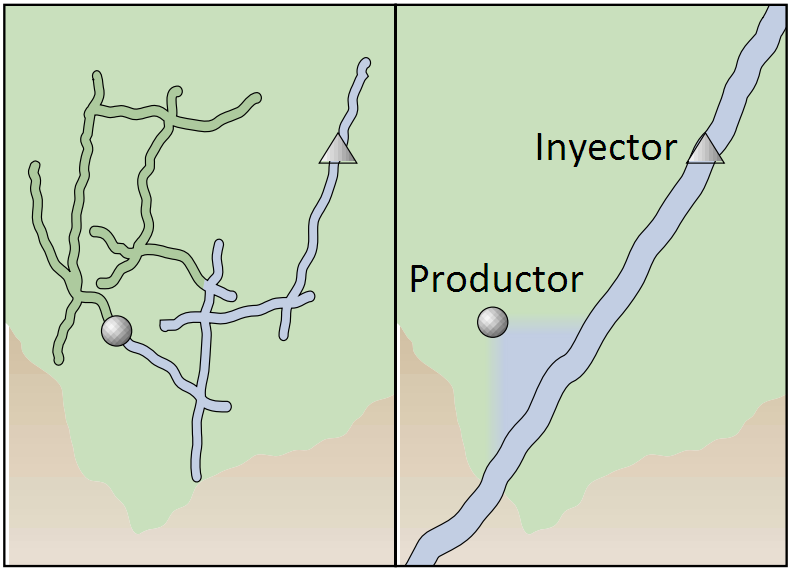
\includegraphics[width=0.65\textwidth]{Graphics/agua5.png}
    \caption[Fracturas de inyector a productor]{Aporte de agua por fallas y fracturas entre pozos inyector y productor. \emph{Adaptado de (\cite{Bailey2000})}.}
    \label{fig:agua5}
\end{figure}

\subsection{Fallas y fracturas desde un acuífero}
El agua puede ser producida desde fracturas que interconectan zonas acuíferas mas profundas con el intervalo disparado (\autoref{fig:agua6}). Estas fracturas pueden ser obturadas cuando no aportan aceite a la producción, sin embargo el reto radica en que no se conoce el tamaño del volumen fracturado. Este caso es mas común en pozos terminados horizontalmente.

\begin{figure}\centering
  \subfloat[pozo vertical]{
    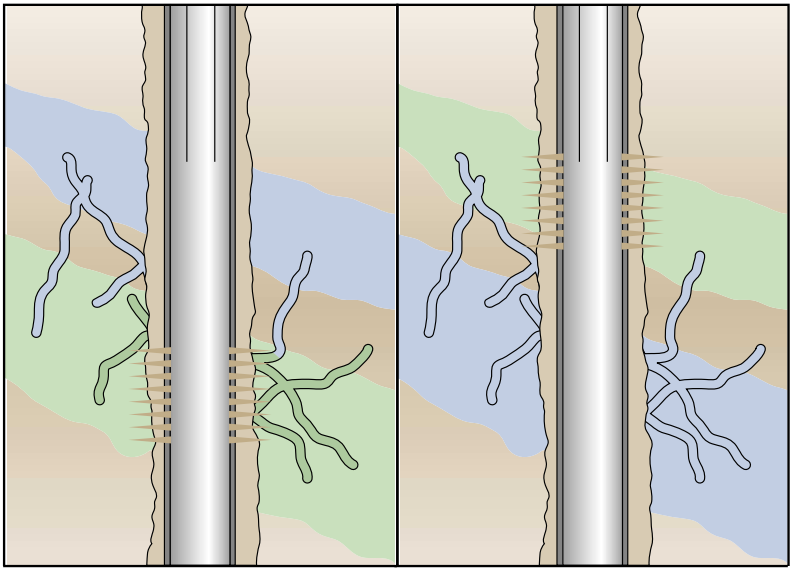
\includegraphics[width=0.45\textwidth]{Graphics/agua6a.png}} \quad
  \subfloat[pozo horizontal]{
    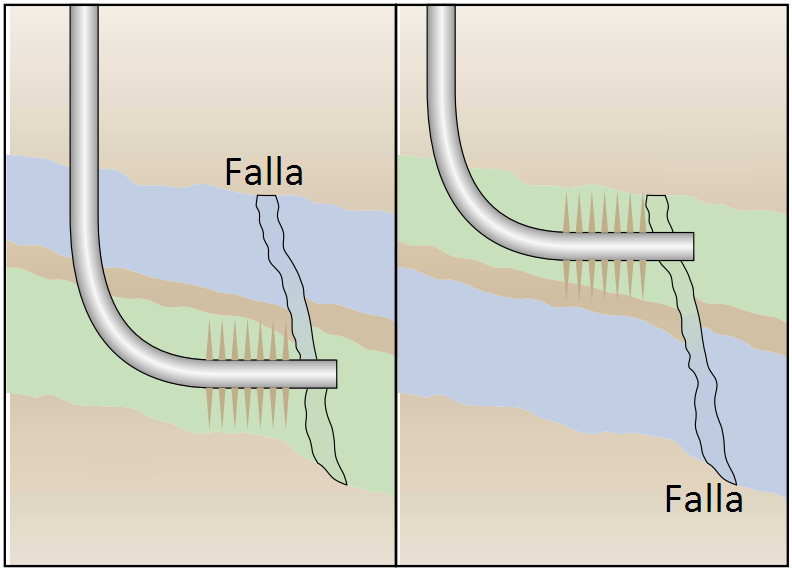
\includegraphics[width=0.45\textwidth]{Graphics/agua6b.png}} 
  \caption[Fallas y fracturas desde un acuifero]{Aporte de agua por fallas y fracturas desde un acuífero mas profundo \textbf{a)} y desde un acuífero mas somero \textbf{b)} . \emph{Adaptado de (\cite{Bailey2000})}.}
  \label{fig:agua6}
\end{figure}

\subsection{Conificación y Dunas}
La conificación es principalmente el resultado del movimiento de los fluidos del yacimiento en la dirección de menor resistencia, equilibrada por una tendencia de los fluidos a mantener la segregación gravitacional. 

En un pozo vertical ocurre a menudo cuando la zona disparada se encuentra cerca del contacto agua aceite en una formación con permeabilidad vertical relativamente alta. Existe un ritmo de producción máximo para no producir agua a través de un cono, pero este siempre es muy bajo para ser económicamente factible. En pozos horizontales este problema es referido como duna o cresta (\autoref{fig:agua7}).

\begin{figure}\centering
    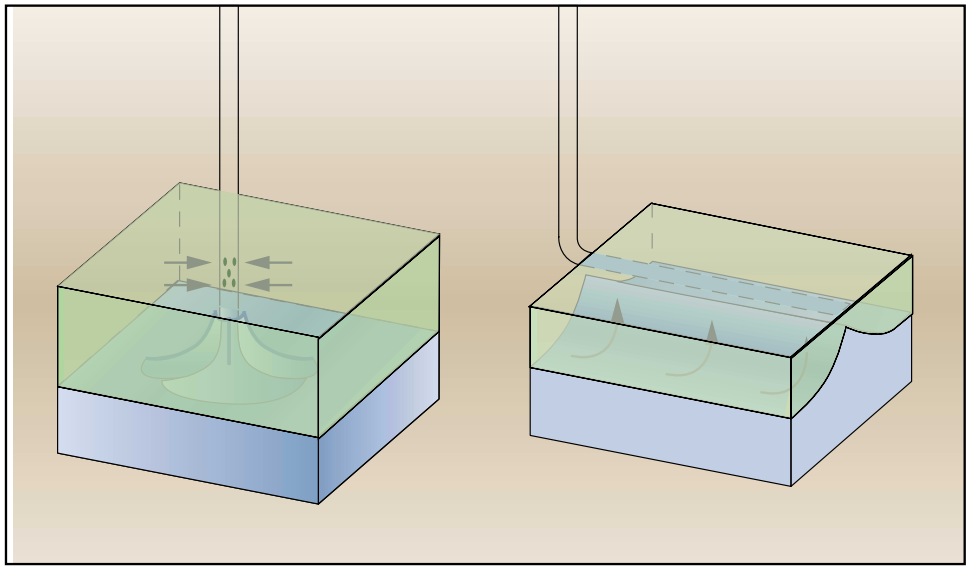
\includegraphics[width=0.65\textwidth]{Graphics/agua7.png}
    \caption[Conificación y dunas]{Conificación de agua en pozos verticales y \emph{dunas} en pozos horizontales. \emph{Adaptado de (\cite{Bailey2000})}.}
    \label{fig:agua7}
\end{figure}

\subsection{Barrido areal deficiente}
Un acuífero o pozo inyector de agua muy cercano a la zona impregnada de aceite a menudo provoca un barrido areal deficiente (\autoref{fig:agua8}). La heterogeneidad de la formación y anisotropía es la principal causa de este problema que es muy frecuente en depósitos de canal en arenas.

\begin{figure}\centering
    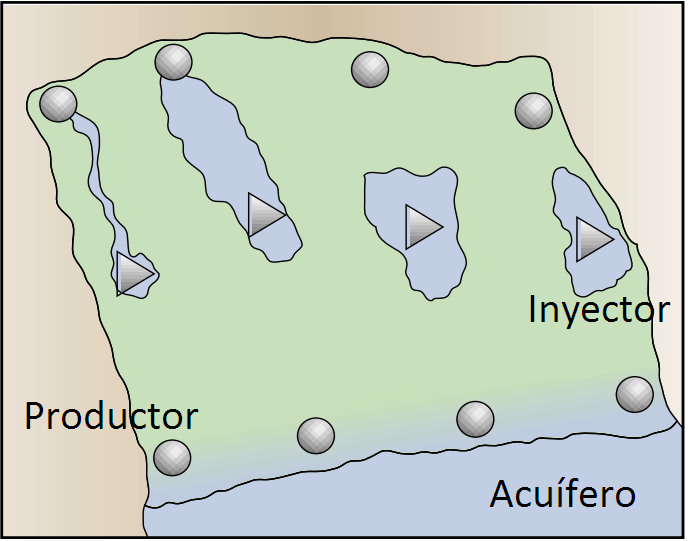
\includegraphics[width=0.63\textwidth]{Graphics/agua8.png}
    \caption[Barrido areal deficiente]{Los pozos productores cercanos al acuífero rápidamente serán invadidos por agua, mientras que las heterogeneidades del yacimiento y la diferencia de permeabilidades entre estratos y facies provoca que el agua no desplace de manera eficiente al aceite hacia los pozos. \emph{Adaptado de (\cite{Bailey2000})}.}
    \label{fig:agua8}
\end{figure}

\subsection{Capa con segregación gravitacional}
En un yacimiento de gran espesor con buena permeabilidad vertical, la segregación gravitacional de fases (agua-aceite) puede provocar un aporte de agua desfavorable hacia el pozo productor. El agua proveniente de un acuífero activo o pozo inyector, se infiltra en la parte baja de la formación permeable barriendo únicamente una parte del aceite del yacimiento al pozo (\autoref{fig:agua9}). Una baja movilidad del aceite y formaciones con texturas sedimentarias mas finas en la parte superior pueden empeorar el problema, pues los efectos viscosos y la segregación favorecen el flujo de agua en la parte baja del yacimiento.

\begin{figure}\centering
    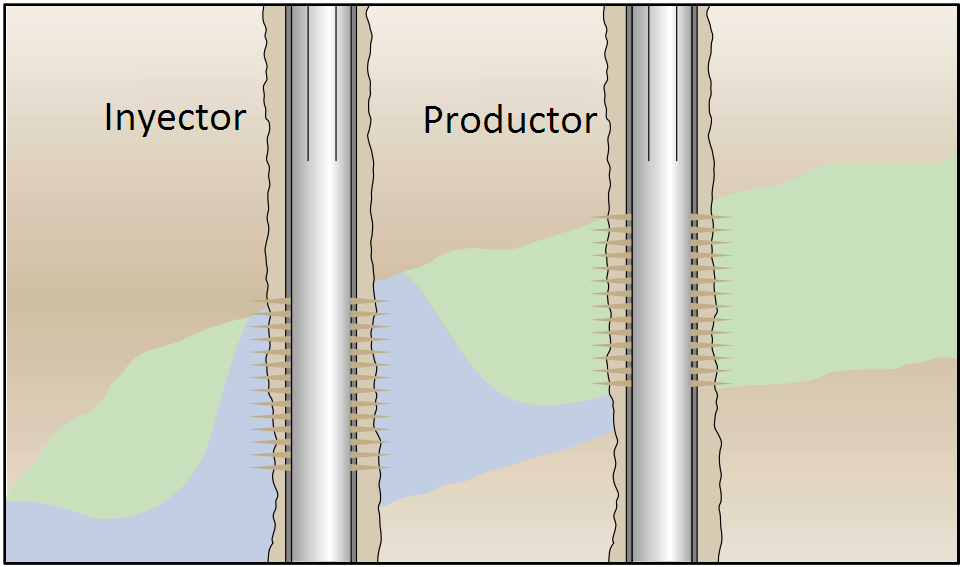
\includegraphics[width=0.65\textwidth]{Graphics/agua9.png}
    \caption[Capa con segregación gravitatacional]{Capa de riego con aporte de agua por debajo del aceite debido a la segregación gravitacional. \emph{Adaptado de (\cite{Bailey2000})}.}
    \label{fig:agua9}
\end{figure}

\subsection{Capa de riego con flujo transversal}
El flujo transversal puede ocurrir en formaciones que presentan capas con alta permeabilidad que no se encuentran aisladas una de otra por barreras impermeables \autoref{fig:agua10}.

\begin{figure}\centering
    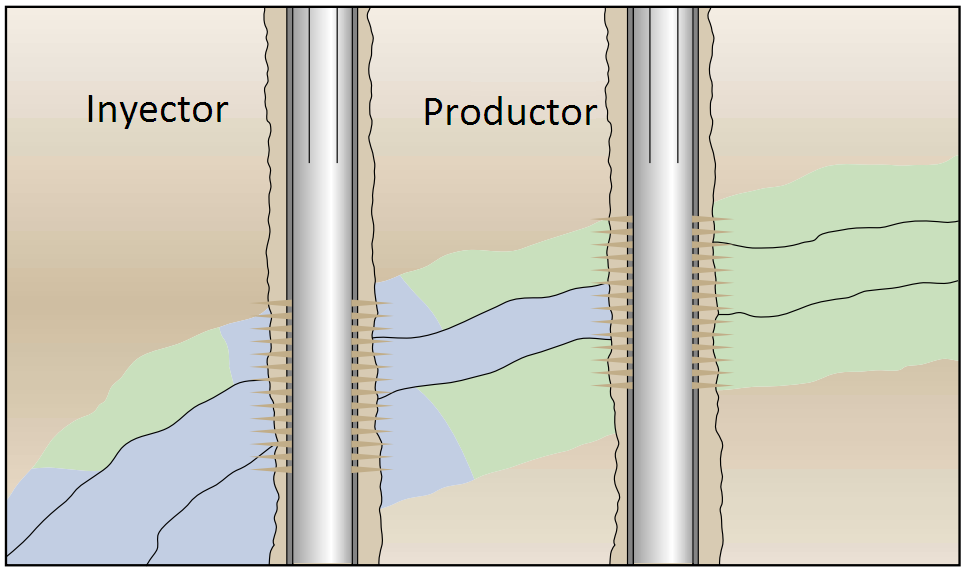
\includegraphics[width=0.65\textwidth]{Graphics/agua10.png}
    \caption[Capa de riego con flujo transversal]{En el caso del flujo transversal al no haber barreras impermeables entre estratos o capas, aislar la capa de riego no resolverá el problema. \emph{Adaptado de (\cite{Bailey2000})}.}
    \label{fig:agua10}
\end{figure}


\section{Técnicas de control y mitigación de la producción de agua}
Existen básicamente tres enfoques distintos para el control de agua producida en exceso, soluciones mecánicas, químicas y operaciones mas complejas y costosas que incluyen cambios en el estado mecánico del pozo o el aparejo de producción. En ocasiones mas de un problema esta presente, por lo que una combinación de técnicas deben ser implementadas.

De manera general \cite{Seright2001} agrupa en tres categorías donde se distingue la problemática a atacar y la solucion recomendada de uno o mas problemas como se muestra en la \autoref{tab:agua1}.

\begin{table} \caption[Categorias: Problemática y tratamiento]{Categorías de problemas de producción de agua excesiva y su tratamiento. Adaptada de (\cite{Seright2001}). }
        \begin{tabulary}{\textwidth}{LL}
            \multicolumn{2}{l}{Categoría \textbf{A} Tratamientos mecánico}\\ 
            \midrule              
             $\bullet$ & Fugas en el revestimiento \\
             $\bullet$ & Canalización detrás del revestimiento\\
        \end{tabulary} 
    \\ \vspace{0.5cm}
        \begin{tabulary}{\textwidth}{LL}
            \multicolumn{2}{l}{Categoría \textbf{B} Tratamiento con geles}\\ 
            \midrule              
            $\bullet$ & Conificación del acuífero a través de una fractura\\
            $\bullet$ & YNF con acuífero asociado \\
            $\bullet$ & Fuga a través del revestimiento \\
        \end{tabulary}
    \\ \vspace{0.5cm}
    \begin{tabulary}{\textwidth}{LL}
        \multicolumn{2}{l}{Categoría \textbf{C} Tratamiento con geles preformados}\\ 
        \midrule              
        $\bullet$ & Fallas o fracturas que cruzan pozos horizontales \\
        $\bullet$ & Una fractura causante de canalización entre dos pozos\\
        $\bullet$ & YNF causando canalización entre dos pozos \\
    \end{tabulary}
    \\ \vspace{0.5cm}
\begin{tabulary}{\textwidth}{LL}
    \multicolumn{2}{l}{Categoría \textbf{D} Casos especiales}\\ 
    \midrule              
    $\bullet$ & Conificación de agua \\
    $\bullet$ & Dunas de agua (pozo horizontal) \\
    $\bullet$ & Aporte de agua por capas de riego\\
\end{tabulary}
    \label{tab:agua1}
\end{table}

\subsection{Soluciones mecánicas}
En muchos de los casos donde el problema se encuentra cercano al agujero de pozo, como fugas detrás del revestimiento o capas de riego sin flujo transversal, se aisla el intervalo por medio de tapones mecánicos o inflables, así como también cementaciones que pueden ser colocadas en agujeros descubiertos o entubados. Los detalles de estas operaciones pueden ser consultados en otros trabajos (\cite{SLB:2014}).

\subsection{Métodos químicos}
Esta categoría consta básicamente de incluye los químicos formadores de geles y en ocasiones su mezcla con cemento (\cite{SLB:2011}).

\begin{description}
    \item[Geles acuosos] Son formados por polímeros sintéticos y geles reticulantes, se utilizan en yacimientos naturalmente fracturados, donde se produce un alto corte de agua a través de las fracturas. Son de peso molecular alto lo cual limita las pérdidas de gel en la matriz y da como resultado viscosidades altas penetrando en las fracturas naturales.
    \item[Geles rígidos] Consisten en un sistema que produce un gel polimérico sintético reticulado de gran fuerza el cual es capaz de penetrar en la matriz antes de gelificarse. Se utiliza cuando se requiere la obstrucción completa de la vecindad del pozo por canalizaciones, canales de alta permeabilidad y abandono de zonas.
    \item[Lechadas selectivas] Estas lechadas están compuestas por cemento microfino suspendido en un medio orgánico (solventes y surfactantes). Esta composición provee la característica de mantenerse en fase líquida, es decir sin adquirir consistencia de fraguado ni de desarrollar gelificación, mientras no entre en contacto con agua. En los canales mojados con aceite esta lechada se mantendrá en estado líquido, lo cual permitirá removerla fácilmente; en cambio al contacto con agua el cemento se empezará gelificar y posteriormente a fraguar.
    \item[Modificadores de la permeabilidad relativa] consiste en un polímero (normalmente catiónico) soluble en salmuera acuosa. La absorción del polímero reduce la sensibilidad  en las arcillas y areniscas al intercambio catiónico, reduciendo la permeabilidad relativa al agua y minimizando el cambio de permeabilidad relativa al aceite.
\end{description}


\section{Sistemas Dispersados}
El concepto de sistema dispersado fue introducido por primera por \cite{Ostwald} y \cite{Weimarn} en su intento por estudiar las propiedades de los coloides. Un sistema dispersado incluye cualquier medio homogéneo, que contiene entidades dispersas de cualquier tamaño y en cualquier estado (\cite{ShortText}). Los coloides y su vez las emulsiones pueden ser contenidos dentro de esta definición. Las propiedades y el comportamiento de estos sistemas esta relacionado con el tamaño y la forma de las partículas dispersas. La primera clasificación para los sistemas dispersados se basaba en el tamaño de las partículas \autoref{tab:coloid1}. Estos límites fueron arbitrariamente escogidos por Ostwald, aunque las propiedades coloidales pueden presentarse en partículas mucho mas grandes de hasta $0.0005 mm$.

 \begin{table} 
 \caption[Sistemas dispersados]{Clasificación de los sistemas dispersados. Adaptada de (\cite{ShortText}).}
     \centering
     \begin{tabulary}{\textwidth \tymin=99.73pt}{L C L}
     \toprule
        \multicolumn{3}{c}{Sistemas Dispersados}\\\midrule%
        Dispersiones gruesas & Dispersiones coloidales & Moléculas pequeñas y átomos\\%
        ~ $>0.1 \mu$ m  & $0.1 \mu$ m - $10 A$  & $< 10 A$ \\%
         ~ \tikzmark{a} & ~ & \tikzmark{b}\\%
     \bottomrule
     \end{tabulary}     
     \label{tab:coloid1}
  \end{table}
  
  \begin{tikzpicture}[overlay, remember picture] 
     \draw[thick,->] (a) -- (b) node[label=right:{\textit{menor tamaño}}]{};
  \end{tikzpicture}

Dado que algunas moléculas, como por ejemplo la celulosa, poseen dimensiones de $0.0015$ mm de longitud, pero $8x10^{-7}$ mm ($8$ A) de espesor, pueden ser clasificadas por su longitud dentro de las dispersiones gruesas, mientras que su espesor está cerca de ser una dispersión molecular. Para sobreponerse a esta problemática una nueva clasificación para los sistemas dispersados (\cite{Staudinger}), fue propuesta para tomar en cuenta el número de átomos que componen a la fase dispersada y no el tamaño de las partículas \autoref{tab:coloid2}.
 
 
  \begin{table}
 \caption[Sistemas dispersados]{\raggedright Propiedades de los sistemas dispersados. Adaptada de (\cite{ShortText}).}
     \centering \footnotesize
     \begin{tabulary}{\textwidth \tymin=99.73pt}{L|L|L}
     \toprule 
        Dispersiones gruesas & Coloides &  Moléculas pequeñas y átomos\\ 
        \midrule              
        Partículas compuestas de más de $10^9$ átomos. &  Partículas compuestas de $10^3$-$10^9$ átomos. & Moléculas que contienen $1$-$10^3$ átomos.\\
        
        Partículas visibles en un microscopio ordinario. &  Partículas son visibles en microscopio electrónico y ultramicroscopio, no detectables en microscopio ordinario. & Invisibles en microscopio electrónico.\\ 
        
        Partículas retenidas en papel filtro ordinario. &  Partículas atraviesan papel filtro pero son retenidas en ultra filtros. &  Atraviesan ultra filtros.\\
        
        Partículas no se dializan ni se difunden. &  Muy poca difusión, solo las partículas mas pequeñas se dializan muy lentamente. &  Rápida difusión y diálisis a través de membranas.\\
     \midrule
     \bottomrule
     \end{tabulary}
     \label{tab:coloid2}
\end{table}
 

\subsection{Coloides}

Si bien los coloides son una clasificación de los materiales muy amplia y no existe una estricta definición, en la literatura actual podemos encontrar definiciones de coloide como:

\begin{description}

\item[(\cite{ShortText})] \protect \raggedright Un coloide en su estructura mas básica consiste de un medio homogéneo con partículas dispersadas dentro de el.
\item[(\cite{ColloidSurface})] Cualquier partícula que posea una dimensión lineal entre $10^{-9}m$ ($10$A) y $10^{-6}m$ ($\mu m$).
\item[(\cite{Drew})] Los coloides son, en general, sistemas que consisten en una sustancia (sólido líquido o gas) finamente dividido y distribuido uniformemente, dentro de una segunda sustancia (sólido líquido o gas).
\item[(\cite{Handbook})] Los coloides son pequeñas partículas rodeadas de fluido con al menos una de sus dimensiones dentro del rango submicrónico y que poseen carga eléctrica superficial.

\end{description}


\begin{figure}
\centering
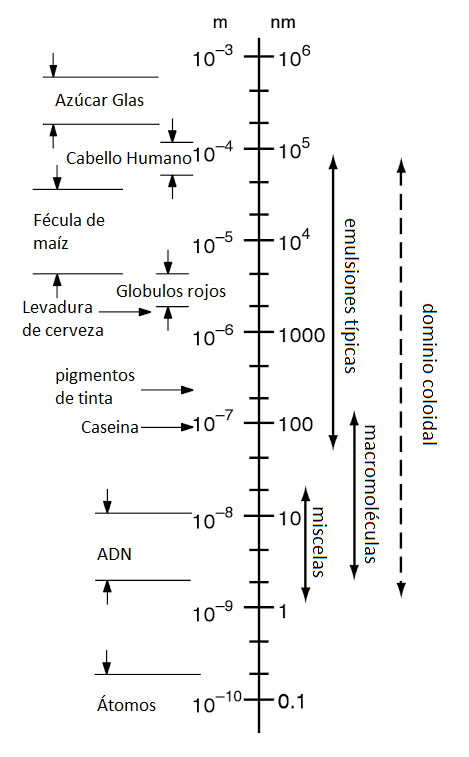
\includegraphics[width=\textwidth]{Graphics/Espectro.png}
\caption[Dominio coloidal]{Dominio coloidal: sus dimensiones y ejemplos típicos de materiales que caen dentro del rango coloidal. Adaptado de (\cite{Cosgrove}). }
\label{fig:Domain}
\end{figure}

De manera que podemos pensar en un coloide como un sistema compuesto por dos sustancias mezcladas de manera especial, donde una de ellas se encuentra dispersa en la otra, donde además la dispersión debe cumplir con ciertos requerimientos de tamaño, en la \autoref{fig:Domain} se muestra el espectro de dimensiones coloidal. Sin embargo en la práctica muchos sistemas con dimensiones que van mas allá del rango de tamaño establecido anteriormente, particularmente las emulsiones, también son incluidos dentro de los coloides, dado que sus características así lo permiten. En este sentido algunos sistemas como las fibras, arcillas y películas delgadas pueden calificar como coloides puesto que alguna de sus dimensiones cae dentro del rango especificado de tamaño y además sus propiedades se asemejan a las del comportamiento coloidal, la (\autoref{fig:Dimensions}) esquematiza este concepto.

% In practice, however, many systems with dimensions beyond that range, in
% particular most emulsions, paints, and aerosols, must also be included under
% the colloid umbrella, since their characteristics allow no other realistic option.
% Other colloidal systems, such as fibers, clays, and thin films, may ‘‘qualify’’ as
% colloids because one or two dimensions fall into the designated range, and
% their properties adhere to the ‘‘rules’’ of colloidal behavior. That concept is
% illustrated schematically in Figure 10.1. Ultimately, the most useful definition
% to use is that if it looks like a colloid and acts like a colloid, it is a colloid,
% regardless of other more restrictive limitations

\begin{figure}
\centering
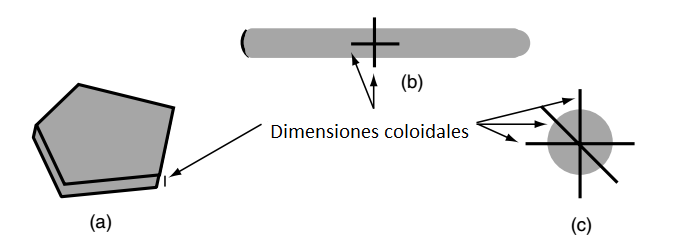
\includegraphics[width=\textwidth]{Graphics/Dimensiones.png}
\caption[Dimensiones coloidales]{Un coloide esta definido básicamente por sus dimensiones. Muchos sistemas con proporciones mucho mas grandes son aun considerados como típicos coloides puesto que al menos una de sus dimensiones cae dentro del rango límite de tamaño como en una placa delgada \textbf{(a)} un cilindro \textbf{(b)} o una gota \textbf{(c)}. Adaptado de (\cite{Drew}). }
\label{fig:Dimensions}
\end{figure}

Los sistemas coloidales pueden ser agrupados en tres clasificaciones generales (\cite{Duncan}):
\begin{description}
  \item[Dispersiones coloidales]
    Son termodinamicamente inestables debido a su alta energía libre superficial, y son sistemas irreversibles en el sentido de que no pueden ser fácilmente reconstituidos después de una separación de fases.
  \item[Soluciones macro moleculares] 
    Son termodinamicante estables y son sistemas reversibles en el sentido de poder reconstituirse con facilidad luego de haber ocurrido la separación del soluto y el solvente.
  \item[Coloides Asociados] 
    % Están relacionados con la formación de estructuras miscelares. Surface-active molecules or surfactants, such as soaps, detergents and lipids, can self-assemble to form multi-molecular aggregates of colloidal size and show the effects of colloidal forces in addition to their individual phase behaviour 
    Las moléculas tensoactivas o surfactantes, como jabones, detergentes y lípidos, pueden auto estructurarse (ensamblarse) para formar agregados multimoleculares de tamaño coloidal y mostrar los efectos de las fuerzas coloidales adicionalmente de su comportamiento de fase individual
    (\cite{Goodwin}).
\end{description}

Algunos ejemplos de coloides encontrados cotidianamente son: leche (grasa liquida dispersada en finas gotas dentro de una fase acuosa), humo (partículas sólidas dispersas en aire), niebla (pequeñas gotas de líquido dispersas en aire), pinturas (pequeñas partículas sólidas dispersas en líquido), geles (moléculas de polímero que, cuando son disueltas en un solvente, proporcionan una estructura semi-sólida a la solución), y hueso (pequeñas partículas de fosfato de calcio dispersas en una matriz sólida de colágeno). Una terminología alrededor del estado de agregación de las sustancias presentes en dispersiones coloidales se muestra en la tabla \autoref{tab:coloid3}.

%\subsection{Clasificación de las dispersiones coloidales}

Dispersiones coloidales con desviación estándar del tamaño medio de partícula menor al $10\%$, se consideran como \emph{monodispersas}. Si la distribución del tamaño medio de partícula es mas amplia, entonces la dispersión es \emph{polidispersa}. Aunque esta clasificación es un tanto arbitraria, los sistemas monodispersos tienen la habilidad de formar cristales coloidales mientras que los polidispersos no pueden. Los sistemas que presentan una distribución del tamaño de partícula bimodal también pueden formar estructuras cristalinas.

% Colloidal dispersions in which the standard deviation on the mean size is less than 10\% of the mean are usually considered to be ‘monodisperse’. If the particle size distribution is broader than this, the dispersion is considered to be ‘polydisperse’. Although this cut-off appears arbitrary, monodisperse systems have the ability to form colloidal crystals whereas polydisperse systems do not. Bimodal systems can also form crystalline structures if the size ratio is suitable. 

\cite{Freundlich} sugiere que las dispersiones coloidales pueden ser divididas en dos clases llamadas \emph{liofílicas} (afinidad al solvente) y \emph{liofóbicas} (repulsivas al solvente) respectivamente, dependiendo de la facilidad con que dicho sistema puede ser redispersado una vez que esta seco.   
% Freundlich, in his classical text on the subject (1926), suggested that colloidal
% dispersions could be divided into two classes, called lyophilic (solvent loving) and
% lyophobic (solvent hating) respectively, depending on the ease with which the system
% could be redispersed if it was allowed to dry out.
\cite{Kruyt} usa la misma clasificación y se refiere a ellos como sistemas reversibles e irreversibles, respectivamente. Esta terminología es particularmente útil cuando se considera el fenómeno de actividad superficial. Las moléculas de materiales tensoactivos tienen una fuerte afinidad por las interfaces, dado que contienen ambas regiones liofílicas y liofóbicas.
% Esta This terminology is particularly useful when one considers the phenomenon of surface activity. The molecules of surface-active materials have a strong affinity for interfaces, because they contain both hydrophilic and lipophiiic (oil-loving) regions.
% De esta manera queda mas clara la naturaleza de esta distinción dado que la prueba máxima para saber que un sistema es liofílico consiste en determinar si el proceso de dispersión ocurre de manera espontánea cuando el disolvente es añadido al coloide.  
% Kruyt (1952) uses the same classification and
% refers to them also as reversible and irreversible systems, respectively. This
% terminology expresses more clearly the real nature of the distinction because the
% ultimate test of whether a system is lyophilic is to determine whether the dispersion
% process occurs spontaneously when the solvent is added to the colloid.
Otro factor que distingue el comportamiento de los sistemas reversibles (liofílicos) e irreversibles (liofóbicos) es la medida en la cual el medio de dispersión (disolvente) es capaz de interactuar con los átomos de la partícula suspendida. Si el solvente puede entrar en contacto con todas o la mayor parte de de esos átomos entonces la energía de solvatación será importante y el coloide debería ser liofílico (reversible) en algún disolvente adecuado. En el caso donde la estructura de las partículas suspendidas (fase dispersa), permite al disolvente entrar en contacto con solo una pequeña fracción de sus átomos, entonces el coloide casi con seguridad será liofóbico (irreversible) en su comportamiento, aun cuando los átomos en su superficie interactúen fuertemente con el disolvente. 

% One contributing factor to the difference in behaviour between reversible(lyophilic) and irreversible (lyophobic) systems is the extent to which the dispersion medium (solvent) is able to interact with the atoms of the suspended particle. If the solvent can come into contact with all or most of those atoms then solvation energy will be important and the colloid should be lyophilic (reversible) in some suitable solvent.

% If the solvent is prevented, by the structure of the suspended particles (i.e. the disperse phase), from coming into contact with any but a small fraction of the atoms of those particles then the colloid will almost certainly be lyophobic (i.e. irreversible) in its behaviour, even if the surface atoms interact strongly with the solvent


  \begin{table}
 \caption[Dispersiones coloidales]{\raggedright Clasificación de las dispersiones coloidales y ejemplos de ellas (\cite{Pashley}).}
     \centering \footnotesize
     \begin{tabulary}{\textwidth}{L|L|L|C}
     \toprule 
        Fase dispersa & Medio &  Nombre & Ejemplos\\ 
        \midrule              
        Líquido & Gas & Aerosol líquido & Nieblas, \emph{sprays}\\
        Sólido & Gas & Aerosol sólido & Humo, polvo\\
        \multicolumn{4}{c}{~}\\
        Gas & Líquido & Espuma & Espumas\\
        Líquido & Líquido & \textbf{Emulsión} & Leche, mayonesa\\
        Solido & Líquido & Suspensión & Tinta\\
        \multicolumn{4}{c}{~}\\
        Gas & Sólido & Espuma sólida & Poliestireno\\
        Líquido & Sólido & Emulsión sólida & Ópalo, perla\\
        Sólido & Sólido & Suspensión sólida & Rubí, mantequilla\\
     \midrule
     \bottomrule
     \end{tabulary}
     \label{tab:coloid3}
\end{table}


% Classification of colloidal systems
% Colloidal systems may be grouped into three general classifications:
% 1. Colloidal dispersions are thermodynamically unstable owing to
% their high surface free energy and are irreversible systems in the
% sense that they are not easily reconstituted after phase separation.
% 2. True solutions of macromolecular material (natural or synthetic)
% are thermodynamically stable and reversible in the sense that they
% are easily reconstituted after separation of solute from solvent.
% 3. Association colloids which are thermodynamically stable (see
% Chapter 4)
%\subsection{Emulsiones}
%
%Las emulsiones son un tipo de dispersión coloidal que de dos líquidos inmiscibles. En una emulsión las gotas de tamaño coloidal formadas de uno de los líquidos (fase dispersa) se encuentran dispersadas dentro de un medio de otro líquido (fase continua). Diferentes clases de emulsiones pueden ser identificadas, entre ellas aceite en agua (\textbf{O/W}), agua en aceite (\textbf{W/O}) y aceite en aceite (\textbf{O/O}) (\cite{Tharwat}).

%\section{Geles}



\section{Conceptos de relevancia en la industria}
Cuando sólo existe un fluido en los espacios porosos de una roca, se considera que solo hay un conjunto de fuerzas activas, que es, la atracción entre la roca y el fluido. En cualquier yacimiento donde esté presente un único fluido, tal como un acuífero, estas fuerzas pueden no ser tan importantes porque la porosidad y la permeabilidad absoluta son en cierta medida suficientes para definir las características de tales depósitos. Sin embargo, cuando hay más de una fase de fluido, es necesario considerar al menos tres conjuntos de fuerzas activas, para un sistema de dos fluidos, las fuerzas a considerar son:
\begin{itemize}
    \item{Fluido1 - Fluido2}
    \item{Fluido1 - Roca}
    \item{Fluido2 - Roca}
\end{itemize}

La existencia de estas fuerzas da lugar a propiedades fundamentales como la tensión interfacial y la mojabilidad. Además la existencia de dos fluidos dentro del espacio poroso introduce otras propiedades como la presión capilar y la permeabilidad relativa. En conjunto estas propiedades son necesarias para describir las características y el potencial de cualquier yacimiento.

Existe una clara dependencia de estas propiedades con la tensión interfacial (mostrada abajo), por lo que se abordan en orden partiendo del concepto mas general.

\begin{figure}[h]
    \centering
    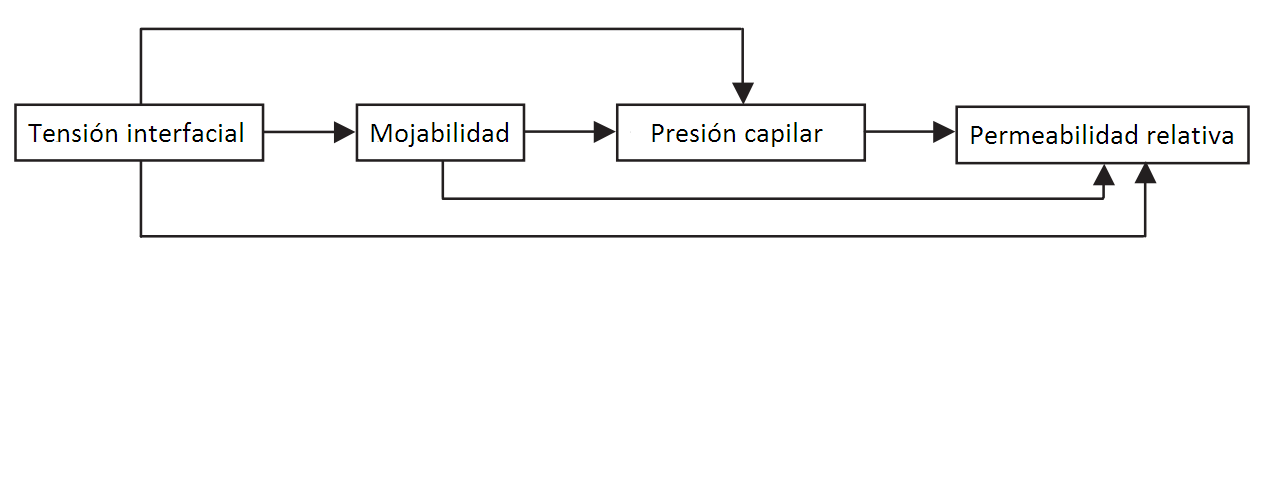
\includegraphics[width=\textwidth]{Graphics/dependencia.png}
%    \caption[Concepto de porosidad]{Dependencia . Adaptado de (\cite{Dandekar}). }
    \label{fig:dependencia}
\end{figure}

\subsection{Porosidad}
Una roca típica de yacimientos como la arenisca es el resultado de granos de arena con diferentes tamaños agrupados como parte del proceso deposicional que forman un consolidado, con espacios vacíos entre granos (\autoref{fig:poro1}). La mayoría de las rocas sedimentarias están conformadas por granos con diámetros que varían en el rango de $0.05$ a $0.25~$ mm, resultando en un promedio de radio de poro (espacios vacíos) de entre $20$ y $200~\mu$m (\cite{Tissot}). Cuanto mayor porosidad posea una roca, esta tendrá mayor cantidad de espacio vacío y por consecuencia mayor capacidad para almacenar los fluidos del yacimiento, es por eso que representa una de las propiedades mas importantes de la roca.

\begin{description}
    \item[Definición] La porosidad ($\phi$) se define como el cociente entre el volumen poroso (espacio vacío) dentro de un roca y su volumen total, expresado en porcentaje.
\end{description}

\begin{equation}
        \phi = \frac{Volumen~ poroso}{Volumen~ total}
\end{equation}

El volumen poroso se refiere a la suma, o el volumen combinado, de todos los espacios de poro presentes en la roca.

\begin{figure}
\centering
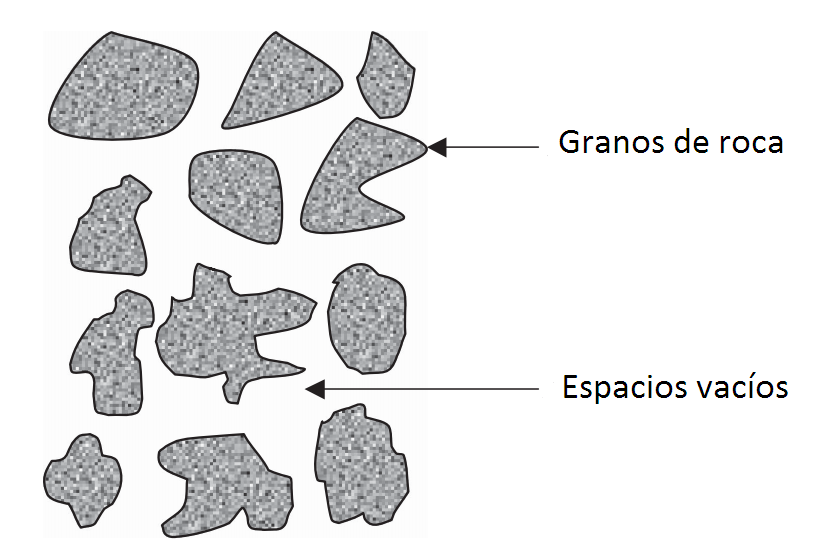
\includegraphics[width=0.7\textwidth]{Graphics/poro1.png}
\caption[Concepto de porosidad]{Representación conceptual del espacio poroso en una roca sedimentaria. Adaptado de (\cite{Dandekar}). }
\label{fig:poro1}
\end{figure}

\subsubsection{Tipos de porosidad}
Algunos de los espacios porosos de una roca pueden estar interconectados con otros poros formando una red, algunos otros pueden estar conectados con poros sin salida, que no conectan con otros poros y también existen espacios porosos que están completamente aislados. Estas características se deben a la variedad de procesos geológicos y deposicionales particulares de cada región y tipo de sedimento, pero en general para las rocas se pueden distinguir tres tipos de poros: interconectados, poros sin salida y poros aislados su representación se muestra en la \autoref{fig:poro2}.

\begin{figure}
    \centering
    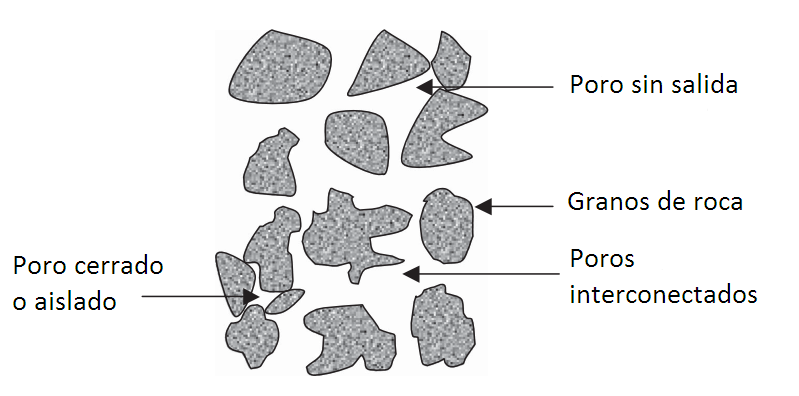
\includegraphics[width=0.9\textwidth]{Graphics/poro2.png}
    \caption[Tipos de porosidad]{Representación conceptual de los tipos de espacio poroso en una roca sedimentaria. Adaptado de (\cite{Dandekar}). }
    \label{fig:poro2}
\end{figure}

En base a estos tres tipos de poros, la porosidad total o absoluta de una roca comprende tanto la porosidad efectiva como la no efectiva en términos de almacenamiento de fluidos.

\subsubsection{Porosidad efectiva}

\begin{description}
    \item[Definición] La porosidad efectiva ($\phi_{EF}$) se define como el cociente de el volumen poroso interconectado y sin salida de una roca entre su volumen total, expresado en porcentaje.
\end{description}

\begin{equation*}
\phi_{EF} = \frac{Vol.~ poros~ interconectados + Vo.~poros~sin salida }{Volumen~ total}
\end{equation*}

Aun cuando la porosidad en algunas rocas carbonatadas es en su mayoría del tipo sin salida, estos poros pueden producir hidrocarburos por medio de la despresurización y expansión del gas.

\subsubsection{Porosidad no efectiva}

\begin{description}
    \item[Definición] La porosidad no efectiva ($\phi_{NOEF}$) se define como el cociente entre el volumen poroso aislado o completamente desconectado de una roca y su volumen total, expresado en porcentaje.
\end{description}

\begin{equation*}
\phi_{NOEF} = \frac{Vol.~ poros~ no conectados }{Volumen~ total}
\end{equation*}

Este tipo de porosidad no es capaz de aportar fluidos durante la producción en un yacimiento.

En general para material con cementación baja o moderada (arenas), la porosidad absoluta será aproximadamente igual a la porosidad efectiva, mientras que para material con muy buena cementación (carbonatos) existirá una diferencia importante debido a que gran parte de la porosidad puede encontrarse completamente aislada del resto.

\subsubsection{Porosidad primaria y secundaria}

Adicionalmente se pueden distinguir dos clasificaciones de porosidad original e inducida, comúnmente referidas como primaria y secundaria. La porosidad original es el resultado de la depositación del material, mientras que la inducida se desarrolla por procesos geológicos que ocurren posterior a la depositación (\cite{Amix}). Ejemplos de porosidad secundaria son las fracturas y vúgulos en rocas carbonatadas mientras que las arenas presentan comúnmente solo porosidad primaria.

\subsection{Permeabilidad} 


\begin{figure}
    \centering
    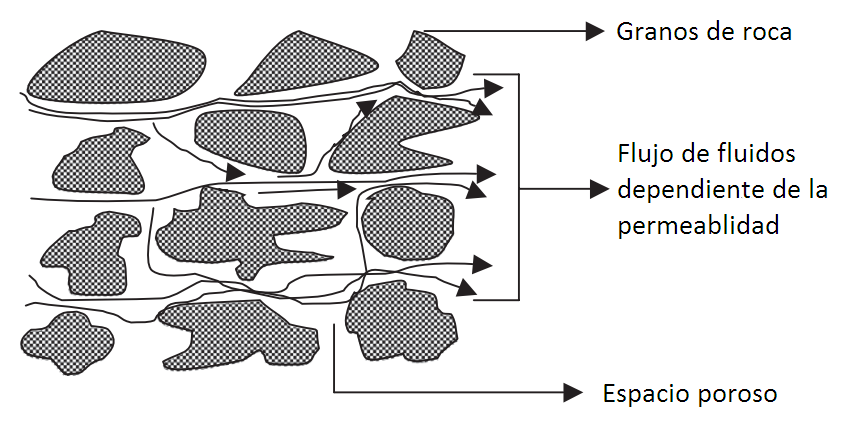
\includegraphics[width=0.9\textwidth]{Graphics/perme1.png}
    \caption[Concepto de Permeabilidad]{Representación conceptual de la permeabilidad de una roca. Adaptado de (\cite{Dandekar}). }
    \label{fig:perme1}
\end{figure}

Esta propiedad ha sido definida de varias maneras por diversos autores (\cite{Dandekar}) como:

\begin{itemize}
    \item La medida de la capacidad de flujo de una roca 
    \item La medida de la capacidad de flujo del medio poroso para transmitir fluidos
    \item La medida de la conductividad de fluido de un medio poroso particular.
    \item La facilidad para fluir o transmitir fluidos a través de una roca que se encuentra completamente saturada con una sola fase de fluido.
    \item La medida del recíproco de la resistencia que el medio poroso ejerce al flujo de un fluido.
    \item La constante de proporcionalidad entre el gasto de flujo de un fluido y el gradiente de presión aplicado.
\end{itemize}


La expresión matemática que define a la permeabilidad fue propuesta por Darcy (cite DARCY) mientras estudiaba el flujo de agua a través de filtros de arena para su purificación, el experimento se muestra en la \autoref{fig:perme2} y cuya única diferencia es la orientación pues el experimento original se llevaba a cabo de manera vertical. 

\begin{figure}
    \centering
    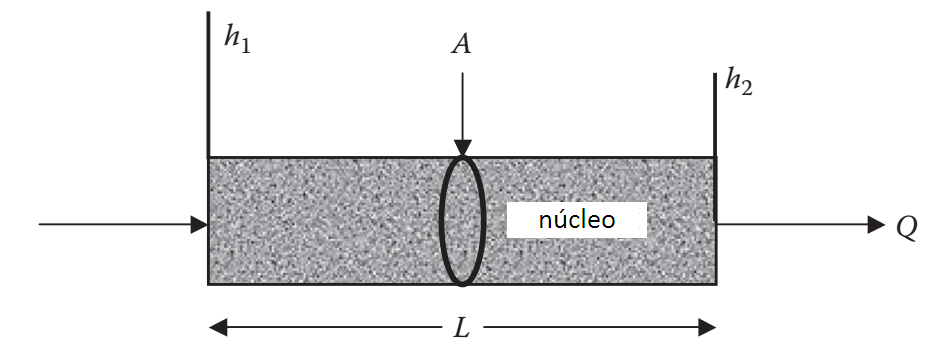
\includegraphics[width=\textwidth]{Graphics/perme2.png}
    \caption[Experimenmto de Darcy]{Experimento de Darcy representando el flujo de un fluido a través de un núcleo de roca . Adaptado de (\cite{Dandekar}). }
    \label{fig:perme2}
\end{figure}

\begin{equation}
Q = KA\frac{h_{1}-h_{2}}{L}
\end{equation}

Donde Q representa el gasto volumétrico a través del núcleo (en $m^{3}/s$ o $ft^{3}/s$), K es la constante de proporcionalidad también definida como conductividad hidráulica (en m/s o ft/s), A es el área transversal del núcleo (en $m^{2}$ o $ft^{2}$), L la longitud del núcleo (en m o ft), y $h_{1}$ y $h_{2}$ representan la carga hidráulica a la entrada y la salida respectivamente (en m o ft).

La ecuación (2) puede ser expresada en término del gradiente de presión d\textit{P} sobre una sección d\textit{L} como:

\begin{gather}
    Q=-KA\frac{dP}{dL}
    \shortintertext{donde}
    dP = \Delta h \rho g
\end{gather}

\textit{d}P es la diferencia entre las presiones corriente arriba y corriente abajo (en $N/m^{2}$), $\Delta h$ es la diferencia entre los gradientes hidráulicos corriente arriba y corriente abajo (m), $\rho$ es la densidad del fluido ($kg/m^{3}$) y g es la aceleración debido a la gravedad ($9.81~m/s^{2}$).
Investigaciones posteriores encontraron que la ley de Darcy puede ser extendida a otros fluidos diferentes al agua, incorporando el término de viscosidad ($\mu$), de manera que la conductividad hidráulica K es expresada como el cociente $k/\mu$, donde k es la \emph{permeabilidad} del medio poroso, lo que permite reescribir la ecuación (3) como:

\begin{equation}
    Q=-\frac{k}{\mu}A\frac{dP}{dL}
\end{equation}
La ecuación (5) puede ser integrada entre los límites de longitud de $0$ a L y de presión a la entrada $P_{1}$ y a la salida $P_{2}$, para el caso del flujo de un fluido como el de la \autoref{fig:perme2} bajo las siguientes suposiciones.

\begin{itemize}
    \item El núcleo se encuentra saturado al 100\% por el fluido.
    \item El flujo es incompresible.
    \item El flujo es horizontal, es estado estacionario y bajo un régimen laminar.
    \item El flujo a través del medio poroso ocurre bajo un régimen viscoso.
    \item El fluido no interacciona con el medio poroso.
\end{itemize}

\begin{gather}
\frac{Q}{A}\int_{0}^{L}dL=-\frac{k}{\mu}\int_{P_{1}}^{P_{2}}dP \\[10pt]
\frac{Q}{A}(L-0) = -\frac{k}{\mu}(P_{2}-P_{1})\\[10pt]
Q=\frac{kA}{\mu L}(P_{1}-P_{2})~~o~~Q=\frac{kA\Delta P}{\mu L}
\end{gather}

La ecuación (8) es comúnmente conocida como la \emph{Ley de Darcy} y se usa extensivamente en cálculos de ingeniería de yacimientos para determinar la permeabilidad absoluta de una roca dentro de un yacimiento. La ecuación (8) representa una combinación de:

\begin{itemize}
    \item La propiedad del medio poroso o la roca de yacimiento esta representado por la permeabilidad k.
    \item La propiedad del fluido esta representado por la viscosidad $\mu$.
    \item La geometría del medio poroso esta representada por el efecto combinado del cociente de su área transversal y longitud A/L.
    \item Las características del flujo están representadas por el gasto Q, y la diferencia de presiones a la entrada y salida $\Delta$P.
\end{itemize}

Aunque las unidades de la permeabilidad en el sistema internacional son de $m^{2}$, la industria petrolera ha adoptado la unidad \emph{darcy} para la permeabilidad en honor del pionero francés. Un medio poroso se dice que posee un darcy de permeabilidad cuando una sola fase de fluido con una viscosidad de $1$ centipoise (cP) satura completamente al medio poroso y fluye a través de este con un gasto de $1cm^{3}/s$ bajo un régimen viscoso y con un gradiente de presión de $1$ atm/cm  en un área transversal de $1cm^{2}$.

\begin{equation}
1~darcy = 1D = \frac{(cm^{3}/s)(cP)}{(cm^{2})(atm/cm)}
\end{equation}

Entre los factores que afectan la permeabilidad absoluta de una roca, encontramos como primer factor el tamaño de grano y la forma. En la \autoref{fig:perme34} (\textbf{a}) se esquematiza un medio poroso hipotético con granos del mismo tamaño y forma en un arreglo uniforme, la figura claramente hace notar que las permeabilidades horizontal y vertical son casi iguales ($k_{H} \approx k_{V}$), dado que sin importar la dirección, las lineas de flujo son similares. Sin embargo al mirar el inciso \textbf{(b)} es obvio que la permeabilidad horizontal es mayor que la vertical, ya que la primera posee lineas de flujo que no presentan restricción al fluido, mientras que en la permeabilidad horizontal las lineas de flujo son tortuosas y significan una mayor restricción.

\begin{figure} \centering
    \subfloat[]{
        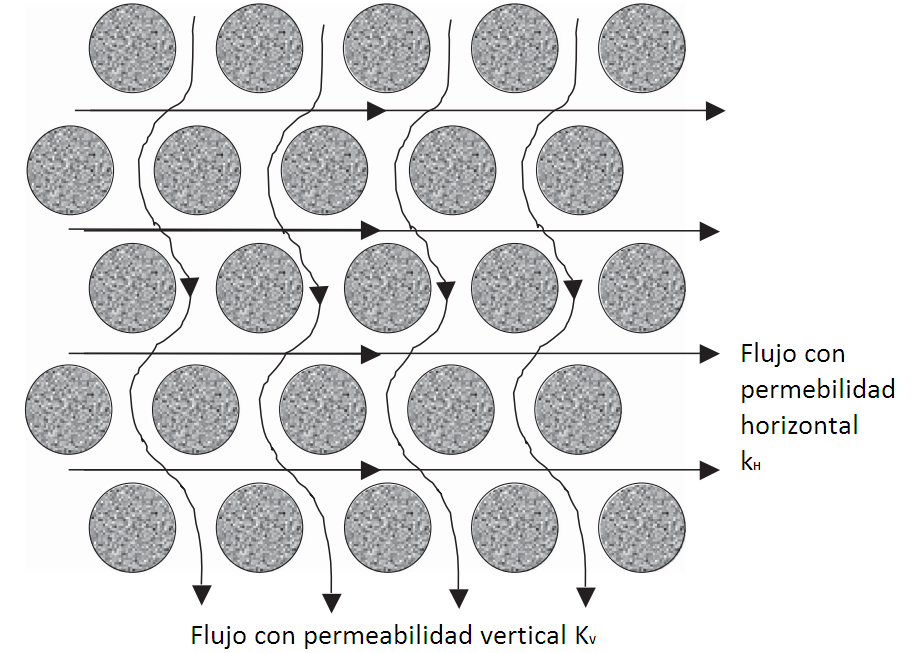
\includegraphics[width=0.8\textwidth]{Graphics/perme3.png} } \quad
    \subfloat[]{
        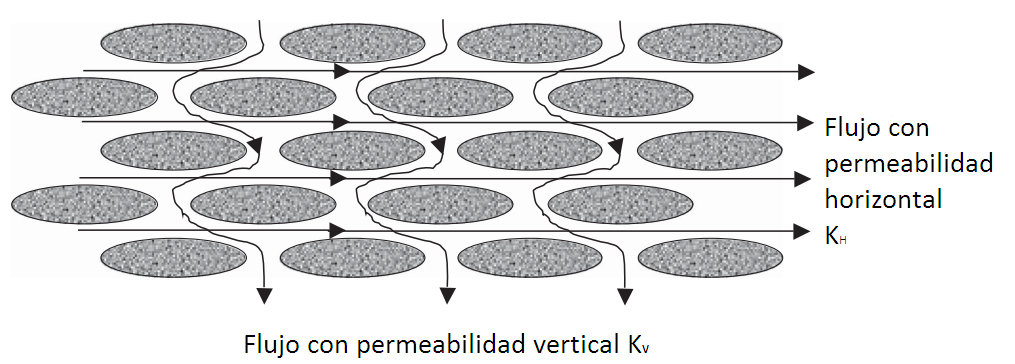
\includegraphics[width=\textwidth]{Graphics/perme4.png} }
    \caption[Permeabilidad vertical y horizontal]{Representación de un medio poroso hipotético formado por: \textbf{(a)} granos de igual tamaño y forma, en un arreglo uniforme ($k_{H}\approx k_{V}$); \textbf{(b)} granos de igual forma aplanados a lo largo en un arreglo uniforme ($k_{H} > k_{V}$). Adaptada de (\cite{Dandekar}).}
    \label{fig:perme34}
\end{figure}

De la misma manera que la porosidad es clasificada en primaria y secundaria, la permeabilidad referida a la matriz cementada de una roca es llamada permeabilidad primaria, mientras que la permeabilidad debido a la presencia de fracturas y canales es conocida como permeabilidad de la fractura o secundaria. En la \autoref{tab:perme1} se muestran las permeabilidades de diferentes tipos de yacimientos alrededor del mundo.

\begin{table}
    \caption[Permebalidades de yacimientos]{Datos de porosidad y permeabilidad de algunas formaciones de arenas y carbonatos alrededor del mundo. Adaptada de (\cite{Dandekar}).}
    \centering \footnotesize
    \begin{tabulary}{\textwidth \tymin=47pt }{L L L L}
        \toprule 
        Campo/Formación & Tipo de Roca &  Porosidad (\%) & Permeabilidad (mD)\\ 
        \midrule              
        Prudhoe Bay, USA & Arena & $22$ & $265$ \\
        Ghawar, Arabia Saudita & Carbonato & $19$ & $617$\\
        Bombay High, India & Carbonato & $15-20$ & $100-250$\\
        Ford Geraldin Unit, USA & Arena  & $23$ & $64$\\
        Elk Hills, USA & Arena & $27-35$ & $100-2000$\\
        Pullai Field, Malasia & Arena & $18-31$ & $300-3000$\\
        Chicontepec, México & Arena & $5-25$ & $0.1-900$\\
        Ekofisk, Noruega & Carbonato  & $30-48$  & $0.25$ \\
        Cretácico superior e inferior, Dinamarca & Carbonato & $15-45$ & $0.01-10$\\
        Daqing, China & Arena & $24.6-26.4$ & $200-1300$\\
        Hassi Messaoud, Algeria & Arena & $7.4$ & $2.5$ \\
        \midrule
        \bottomrule
    \end{tabulary}
    \label{tab:perme1}
\end{table}


\subsection{Saturación}
Mientras que la porosidad representa el la máxima capacidad de una roca para alojar fluidos, la saturación del espacio poroso, cuantifica cuanta de esa capacidad de almacenamiento está realmente ocupada por alguna fase fluida, es decir como se encuentra distribuida o repartida esa capacidad entre las tres fases de fluidos de un yacimiento: agua aceite y gas. Las saturaciones iniciales de fluido, que se definen como las fracciones del espacio poroso ocupado por gas aceite y agua de formación (ecuaciones (10-12)), son los factores clave para determinar la cantidad de hidrocarburos en el yacimiento.
 
 \begin{gather}
    S_{g}=\frac{volumen~ de~ gas}{volumen~ de~ poros}\\[10pt]
    S_{o}=\frac{volumen~ de~ aceite}{volumen~ de~ poros}\\[10pt]
    S_{w}=\frac{volumen~ de~ agua}{volumen~ de~ poros}\\[20pt]
    S_{g}+S_{o}+S_{w}=1.0
 \end{gather}
Donde $S_{g}$, $S_{o}$ y $S_{w}$ son las saturaciones de gas, aceite y agua expresadas en porcentaje o fracción respectivamente. Siempre debe cumplirse que la suma de los volúmenes saturados de alguna fase es igual al total del volumen de poros de la roca ecuación (13). Adicionalmente existen tres casos especiales de saturación de fluidos, que juegan un papel importante para entender el flujo multifásico de fluidos en medios porosos.

\subsubsection{Saturación de gas crítica}
Partiendo del hecho de que los yacimientos de hidrocarburos existen en condiciones de presión y temperatura elevadas y que normalmente el gas hidrocarburo se encuentra disuelto en la fase líquida. Luego de iniciada la producción del yacimiento, la presión de este comienza a declinar mientras la temperatura permanece constante, este cambio en la presión tiene como consecuencia la evolución de una fase gaseosa (la saturación de gas comienza a aumentar desde cero) cuando la presión alcanza un cierto límite de solubilidad conocido como la \emph{presión de saturación} o \emph{punto de burbuja}. La saturación de la fase gas sigue incrementándose mientras que la presión del yacimiento sigue declinando, sin embargo permanece inmóvil o atrapada, hasta que la saturación excede un cierto límite conocido como \emph{saturación de gas crítica} ($S_{gc}$). La fase gaseosa entonces comienza a moverse por encima de esta saturación de gas crítica. Este fenómeno es atribuido al proceso mediante el cual la fase gaseosa se hace continua a través del sistema para comenzar a moverse (\autoref{fig:satgas}).

\begin{figure}\centering
    \subfloat[$S_{g}=0$]{
        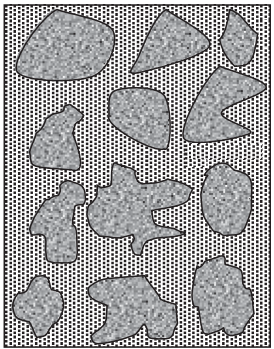
\includegraphics[width=0.3\textwidth]{Graphics/satgasa.png} } \quad
    \subfloat[$S_{g}>0$]{
        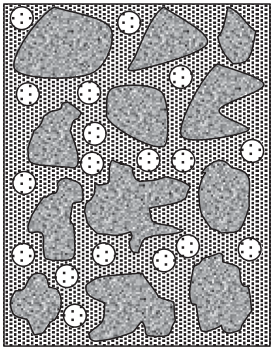
\includegraphics[width=0.3\textwidth]{Graphics/satgasb.png} } \\
    \subfloat[$S_{g} < S_{gc} $]{
        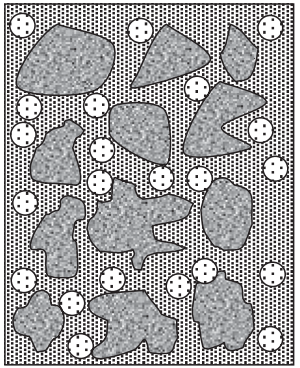
\includegraphics[width=0.3\textwidth]{Graphics/satgasc.png} } \quad
    \subfloat[$S_{g} \ge S_{gc}$]{
        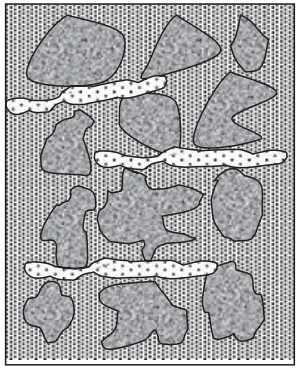
\includegraphics[width=0.3\textwidth]{Graphics/satgasd.png} } \\
    \caption[Saturación de gas crítica]{Representación de los eventos que llevan a la fase gaseosa a la saturación crítica de gas. Adaptada de (\cite{Dandekar})}
    \label{fig:satgas}
\end{figure}

\subsubsection{Saturación residual de aceite}
Esta saturación ($S_{or}$) refiere al aceite remanente en el espacio poroso después de un proceso de desplazamiento. Esta puede ser la saturación de aceite remanente en el yacimiento luego de concluida la explotación primaria. También puede referirse a la saturación de aceite al final de un proceso de recuperación por desplazamiento con gas o agua. Esta saturación también puede ser obtenida en laboratorio en núcleos de roca mediante un proceso de desplazamiento con gas o agua.

\subsubsection{Saturación de agua irreductible}
Los términos \emph{saturación de agua congénita}, \emph{saturación de agua crítica} y \emph{saturación de agua irreductible}, ($S_{wi}$) se encuentran frecuentemente intercambiados en la literatura para hacer referencia al valor de la saturación de agua, al cual la fase agua permanece inmóvil. 

En la mayoría de los yacimientos, los fluidos contenidos han alcanzado un estado de equilibrio, por lo que se han segregado en su mayoría de acuerdo a sus densidades, esto es, gas encima del aceite y este por encima del agua. Se da por hecho que la roca almacenadora se encontraba inicialmente saturada de agua, antes de la migración y entrampamiento de los hidrocarburos (cita). Dado que existe una oposición entre las fuerzas capilares y gravitacionales, la segregación entre las fases no se completa y la saturación de agua se encuentra distribuida a lo largo de las zonas de gas y aceite como se muestra en la \autoref{fig:satagua1}. En estas zonas la saturación de agua se reduce hasta un mínimo, que es la saturación irreductible $Sw_{i}$.
Las fuerzas que retienen esta agua en las zonas de gas y aceite son conocidas como fuerzas capilares y son de importancia debido al tamaño capilar de los poros en la roca. La saturación irreductible de agua depende tanto de la permeabilidad, litología y altura sobre el nivel de la zona invadida por agua, por lo que no se encuentra uniformemente distribuida en el yacimiento.

\begin{figure}
    \centering
    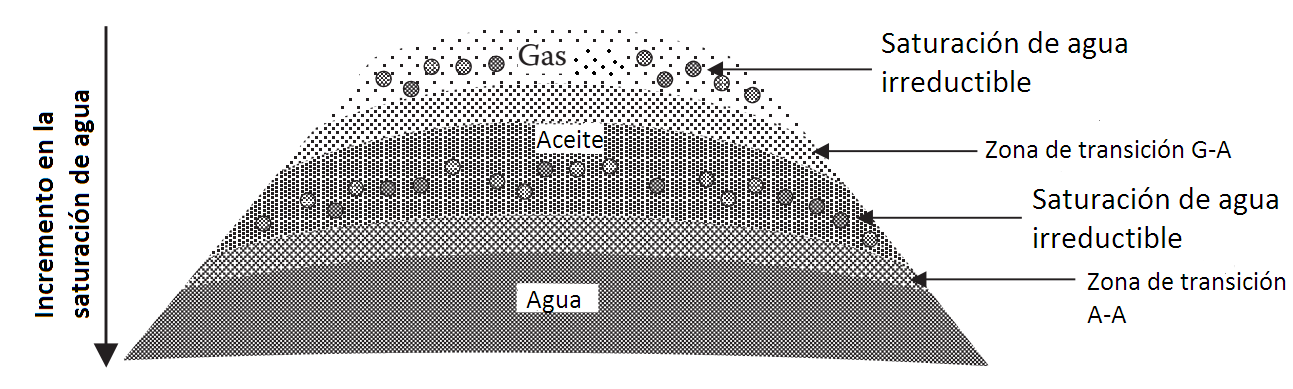
\includegraphics[width=\textwidth]{Graphics/satagua1.png}
    \caption[Saturación de agua irredcutible]{Representación de la saturación de agua irreductible en un yacimiento hipotético. Adaptada de (\cite{Dandekar}). }
    \label{fig:satagua1}
\end{figure}

\subsection{Tensión interfacial}

Para definir este concepto hay que considerar un sistema formado por dos fluidos inmiscibles, agua y aceite (\autoref{fig:tension1}). Una molécula de agua o aceite que se encuentra en el seno del fluido, lejos de la interfase, se encuentra rodeada por otras moléculas de aceite o agua, de esta manera la fuerza de atracción resultante sobre la molécula es igual a cero dado que es \emph{arrastrada} en todas las direcciones. En contraste una molécula en la interfase presenta, tanto una fuerza de atracción ejercida por las moléculas de aceite por encima de la interfase, como atracción por parte de las moléculas de agua bajo esta. Las fuerzas resultantes no están balanceadas debido a que las magnitud de las fuerzas en cada lado de la interfase (arriba y abajo) son distintas, y esto da origen la tensión interfacial.
\begin{description}
    \item[Definición] La tensión interfacial ($\sigma$) es una medida de la energía específica de superficie entre dos fases inmiscibles de diferente composición. Dicho de otra manera es la medida de la energía requerida para formar una unidad de área de interfase entre dos fluidos inmiscibles.
\end{description}
La tensión interfacial tiene dimensiones de fuerza por unidad de longitud expresadas comúnmente en mN/m o $10^{-3}$N/m (dyna/cm).
\begin{figure}
    \centering
    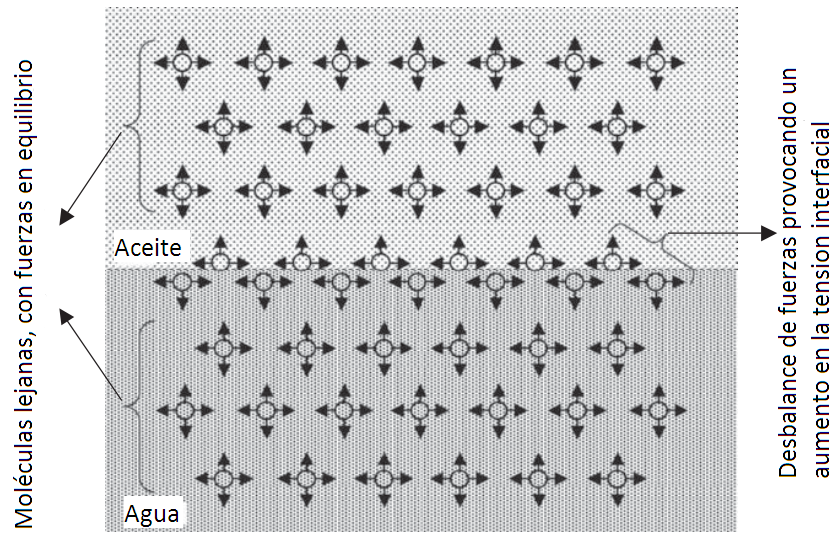
\includegraphics[width=0.8\textwidth]{Graphics/tension1.png}
    \caption[Tensión interfacial]{Representación del concepto de tensión interfacial. Adaptada de (\cite{Dandekar}).}
    \label{fig:tension1}
\end{figure}

\subsubsection{Medición de la tensión interfacial mediante gota pendiente}
Existen diversas técnicas para medir la tensión interfacial, sus características y cualidades se pueden encontrar descritas en el trabajo de \cite{Drelich2002}. El método de la gota pendiente es por mucho el mas simple en términos de instrumentación y versátil. El sistema experimental para medir tensión interfacial por el método de la gota pendiente se compone básicamente por una cámara, una fuente de luz y una aguja (\autoref{fig:dropsystem}).
\begin{figure}
    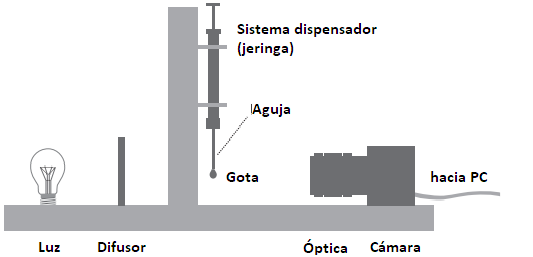
\includegraphics[width=0.8\textwidth]{Graphics/dropsystem.png}
    \caption[Sistema de medicion IFT]{Esquema que muestra el sistema experimental básico para la medición de tensión interfacial por el método de la gota pendiente. Adaptada de (\cite{Berry2015}).}
    \label{fig:dropsystem}
\end{figure}
\subsubsection{Teoría}
Si una gota de líquido se encuentra colgando de la aguja de una jeringa, entonces se asume que tendrá una forma característica de la cual se puede determinar su tensión superficial. La fuerza de gravedad que actúa sobre la gota, dependiendo de su altura, equilibran la presión de Laplace la cual está esta determinada por la curvatura del contorno de la gota. La presión de Laplace está definida en la siguiente expresión conocida como la ecuación de Young-Laplace:
\begin{equation}
\Delta p = \sigma \left( \frac{1}{r_{1}} + \frac{1}{r_{2}} \right)
\end{equation}
Esta expresión describe la diferencia de presión entre el interior y el exterior de una gota que posee como principales radios de curvatura a $r_{1}$ y $r_{2}$. Si la fuerza de gravedad es la única fuerza adicional que actúa sobre la gota, el cambio en la presión puede definirse como $\Delta P = \Delta P_{0}+\Delta \rho gz$, donde $\Delta \rho$ es la diferencia de densidad entre la fases. Utilizando un cambio en el sistema de coordenadas cilíndricas representado en la \autoref{fig:drop}, la ecuación de Young-Laplace se convierte en un sistema de tres ecuaciones diferenciales ordinarias en términos de la longitud de arco $s$ medido desde el apéndice de la gota,
\begin{figure}\centering
    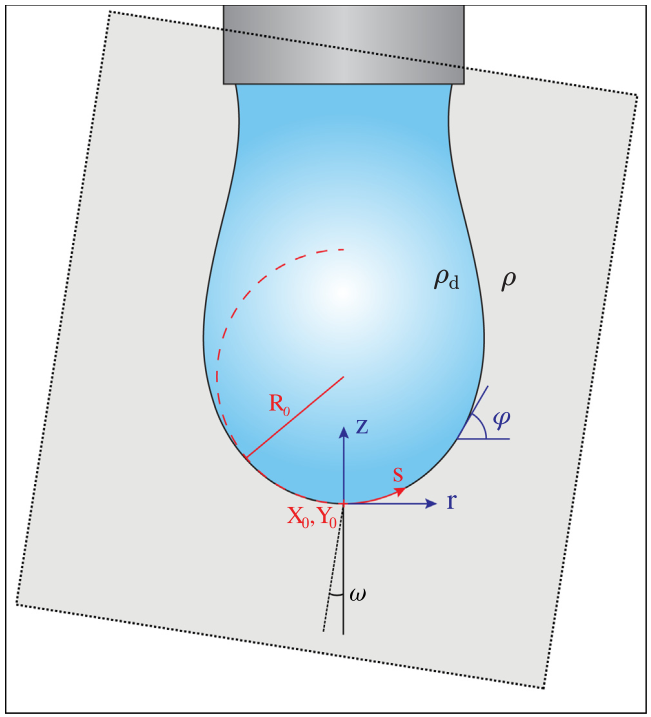
\includegraphics[width=0.6\textwidth]{Graphics/Pendant_drop.png}
    \caption{Esquema de una gota pendiente de una aguja de jeringa, la región sombreada representa el área de imagen capturada por la cámara que no necesariamente se encuentra alineada perfectamente con la gota. Adaptada de (\cite{Berry2015}).}
    \label{fig:drop}
\end{figure}
\begin{eqnarray}
\frac{d\psi}{d\bar{s}} & = & 2-Bo*\bar{z}-\frac{sin(\psi)}{\bar{r}}\\
\frac{d\bar{r}}{d\bar{s}} & = & cos(\psi) \\
\frac{d\bar{z}}{d\bar{s}} & = & sin(\psi)
\end{eqnarray}
la línea indica que se trata de cantidades adimensionales escaladas por $R_{0}$, que es el radio de curvatura en el apéndice de la gota. \emph{Bo} en la ecuación (15) se refiere al número de Bond (\autoref{eqn:bond}).
\begin{equation}
Bo \simeq \frac{\Delta \rho g R_{0}^{2}}{\sigma}
\label{eqn:bond}
\end{equation}
Si el número de Bond asociado con la gota pendiente puede ser determinado junto con el radio de la gota $R_{0}$ en el apéndice, la tensión interfacial $\sigma$ puede obtenerse con la ecuación ($18$). Las condiciones de frontera asociadas son 
\begin{equation}
\bar{r}=0 ,~~ \bar{z}=0,~~ \psi=0 ~~~con~~~ \bar{s}=0
\end{equation}

\subsection{Mojabilidad}%
Dentro de un yacimiento es necesario tomar en consideración las fuerzas que se encuentran activas en la interfase entre líquidos y sólidos, dado que los fluidos de producción, se encuentran necesariamente en contacto con la superficie de la roca. La mojabilidad es un parámetro que determina algunas propiedades del yacimiento como la distribución de aceite agua y gas dentro del yacimiento así como la permeabilidad relativa y la presión capilar.

\begin{description}
    \item[Definición] La mojabilidad es la habilidad de un fluido de esparcirse sobre una superficie sólida en presencia de otro fluido.
\end{description}

Si consideramos la definición anterior, sabemos que la mojabilidad posee un carácter multifásico, dado que se necesitan al menos dos fluidos, con uno de ellos presentando una mayor afinidad hacia la superficie sólida con la que hacen contacto ambos.

La tendencia de un fluido a esparcirse puede ser expresada en términos de la \emph{tensión de adhesión} ($A_{T}$) . La tensión de adhesión es una función de la tensión interfacial y determina la tendencia de mojabilidad de un sistema roca-fluido. Para un sistema de dos fluidos inmiscibles en contacto con una superficie mineral (\autoref{fig:moja1}) la tensión de adhesión se define como:

\begin{figure}
    \centering
    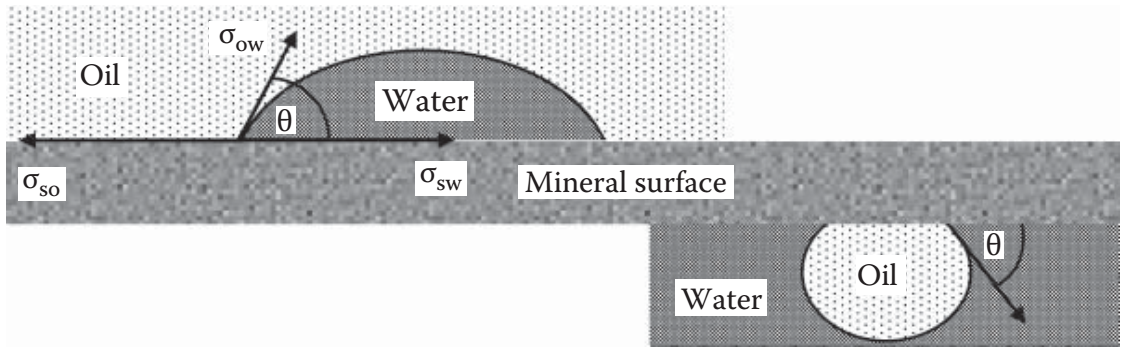
\includegraphics[width=0.9\textwidth]{Graphics/moja1.png}
    \caption[Mojabilidad]{Representación de un sistema de dos líquidos inmiscibles (aceite y agua) en contacto con una superficie mineral. Adaptada de (\cite{Dandekar}).}
    \label{fig:moja1}
\end{figure}

\begin{equation}
A_{T}=\sigma_{SO}-\sigma_{SW}
\end{equation}
Donde $\sigma_{SO}$ es la tensión interfacial entre el sólido y la fase fluida mas ligera (aceite para el caso mostrado) y $\sigma_{SW}$ la tensión interfacial entre el sólido y la fase mas densa (agua para el caso mostrado).

El ángulo de contacto $\theta$ puede varias de $0\degree$ a $180\degree$. Por definición el coseno del ángulo $\theta$ es:

\begin{equation}
cos(\theta_{OW})= \frac{\sigma_{SO}-\sigma_{SW}}{\sigma_{OW}}
\end{equation}

Combinando las ecuaciones (14) y (15):

\begin{equation}
A_{T}=\sigma_{OW}~cos(\theta_{OW})
\end{equation}

Para determinar la tensión de adhesión y definir la mojabilidad del sistema roca-fluido
es necesario conocer el valor de la tensión interfacial entre agua-aceite, y la medida del ángulo de contacto. Un valor de tensión de adhesión positivo indica que la fase mas densa moja preferentemente a la superficie sólida, mientras que un valor negativo indica una preferencia de la fase menos densa a mojar la superficie mineral.

\subsection{Presión capilar}%
La presión capilar existe en un yacimiento siempre que sus poros (de tamaño capilar) se encuentren saturados de dos o más fases inmiscibles fluidas. La frontera entre dos fases inmiscibles presentes en un medio poroso presenta una cierta curvatura debido a la tensión interfacial entre ambos fluidos (\cite{Leverett}). La forma de la curvatura depende de las propiedades de los fluidos y el tamaño de los poros. Es la forma de la curvatura en la interfase lo que da lugar a una diferencia de presión de un lado a otro de la interfase, llamada \emph{presión capilar} ($P_{c}$). Esto significa que cada uno de los fluidos inmiscibles tiene una presión que es distinta de la del otro. 

La presión en la fase no mojante es mayor con respecto de la presión en la fase mojante y por tanto la interfase es curva y convexa respecto a la fase no mojante. Lo anterior puede expresarse de la siguiente manera:

\begin{gather*}
\begin{gathered}
presion~capilar~ = ~presion~fase~no~mojante \\ - ~presion~fase~mojante
\end{gathered} \\
P_{c}=P_{nw}-P_{w}
\end{gather*}


Basado en la altura de líquidos dentro de tubos capilares (\cite{Amix}) desarrolló una serie de ecuaciones que describen la presión capilar en función de la tensión interfacial, el tamaño de poro y la mojabilidad. Si miramos el esquema de la \autoref{fig:capilar1} podemos plantear un balance de fuerzas, dado que el sistema se encuentra en equilibrio, para relacionar la altura del fluido dentro del capilar con el radio, la diferencia de densidades entre el aire y el líquido y la aceleración de la gravedad:

\begin{figure}
    \centering
    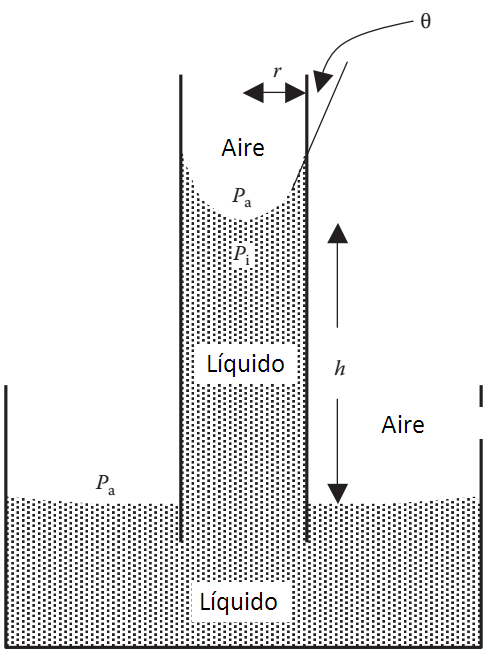
\includegraphics[width=0.6\textwidth]{Graphics/capilar1.png}
    \caption[Presión Capilar]{Esquema que representa las relaciones entre las presiones dentro de un tubo capilar. Adaptada de (\cite{Dandekar}).}
    \label{fig:capilar1}
\end{figure}

\begin{gather}
Fuerza~arriba=2\pi rA_{T} \\[10pt]
Fuerza~abajo=\pi r^{2} h (\rho_{l}-\rho_{a}) g
\end{gather}

Donde $A_{T}$ es la tensión de adhesión (N/m), r es el radio del tubo capilar (m), h es la altura del fluido en el capilar (m), $\rho_{l}$ y $\rho_{a}$ son las densidades del líquido y del aire respectivamente (Kg/$m^{3}$) y g es la aceleración de la gravedad (m/$s^{2}$).

\begin{gather}
2\pi r A_{T} = \pi r^{2} h (\rho_{l}-\rho_{a}) g \\[10pt]
h= \frac{2\pi r A_{T}}{\pi r^{2}(\rho_{l}-\rho_{a}) g}=\frac{2 A_{T}}{r (\rho_{l}-\rho_{a}) g}
\end{gather}

Sin embargo si consideramos la definición de tensión de adhesión, $A_{T} = \sigma_{al}~cos(\theta_{al})$; entonces

\begin{equation}
h=\frac{2 \sigma_{al}~cos(\theta_{al})}{r(\rho_{l}-\rho_{a})g}
\end{equation}

Ahora por definición de presión capilar, una diferencia de presión existe de la interfase líquido aire y puede expresarse como:

\begin{equation}
P_{c}=P_{a}-P_{l}=(\rho_{l}-\rho_{a})gh
\end{equation}

Si combinamos las ecuaciones (23) y (24) obtenemos la ecuación de la presión capilar en términos de las fuerzas de superficie, mojabilidad y tamaño capilar:

\begin{equation}
P_{c} = (\rho_{l}-\rho_{a}) g \frac{2 \sigma_{al}~cos(\theta_{al})}{r(\rho_{l}-\rho_{a}) g} = \frac{2 \sigma_{al} cos~(\theta_{al})}{r}
\end{equation}

De manera general las fuerzas capilares en un yacimiento son la manifestación del efecto de la tensión interfacial, mojabilidad y tamaño de poro del sistema roca-fluido. Las fuerzas capilares son las causantes del entrampamiento de los hidrocarburos en la roca. Un yacimiento antes de la explotación se encuentra en equilibrio capilar-gravitacional. Este equilibrio se manifiesta por medio de una distribución de la saturación de fluidos particular de cada sistema. Por ejemplo en la migración de los hidrocarburos hacia una formación saturada por agua (acuífero) el petróleo entrampado en el yacimiento representa un equilibrio entre la gravedad que intenta moverlo hacia arriba y las presiones capilares que se oponen (\cite{Leverett}). 

Las fuerzas capilares juegan un papel importante en el flujo de dos fluidos inmiscibles en un medio poroso, puesto que la presión capilar debe ser vencida para que una burbuja de aceite o gas pueda fluir a través del pequeño diámetro de un poro. Por ejemplo se necesitan mas de $1480$ psi para hacer fluir una gota esférica de aceite a través de un diámetro de poro de $0.01~\mu$m, asumiendo que la roca se encuentra saturada por agua y que la tensión interfacial agua-aceite es de $25~\mu$N/m.


\subsection{Permeabilidad Relativa}%

Para extender la ley de Darcy al flujo simultaneo de dos o mas fluidos en un medio poroso, es necesario incluir el concepto de \emph{permeabilidad efectiva} de cada fase, en lugar de la permeabilidad absoluta definida anteriormente. La permeabilidad efectiva es función de la saturación de fluido, las características de mojabilidad del medio y de la geometría de los poros. Por lo anterior es necesario además, especificar la saturación del fluido para definir su permeabilidad efectiva. Dada la gran cantidad de combinaciones de saturaciones de dos o más fluidos dentro de un medio poroso, los datos de permeabilidad son reportados como \emph{permeabilidad relativa} ($K_{r}$) en lugar de permeabilidad efectiva \autoref{fig:satrel}.

\begin{figure}
    \centering
    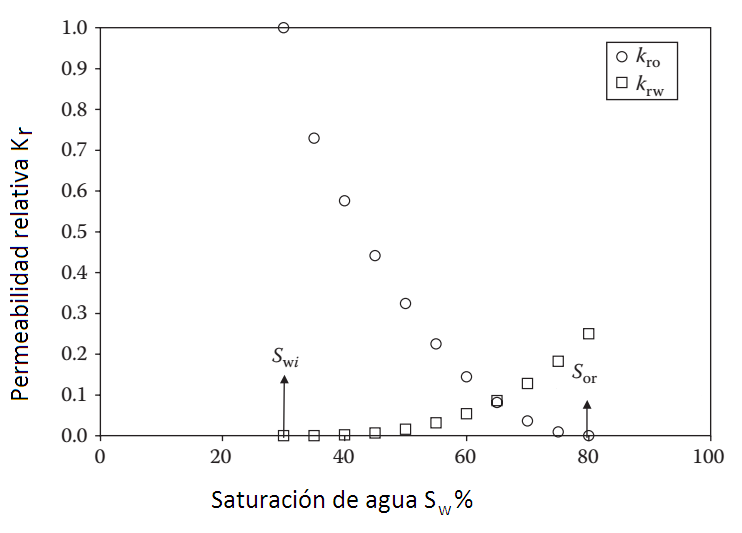
\includegraphics[width=0.8\textwidth]{Graphics/satrel.png}
    \caption[Saturación relativa]{Curva típica de saturación relativa para agua y aceite. Adaptada de \cite{Dandekar}.}
    \label{fig:satrel}
\end{figure}

\begin{description}
    \item[Definición]La permeabilidad relativa se refiere a la proporción entre la permeabilidad efectiva de un fluido con respecto de la permeabilidad absoluta del medio (ecuación (24)). La permeabilidad relativa es una medida de la conductividad de un fluido en el medio poroso, cuando este se encuentra saturado con otros fluidos (\cite{Dandekar}). 
\end{description}

\begin{equation}
K_{r}=\frac{K_{e}}{K}
\end{equation}

Donde $k_{r}$ es la permeabilidad relativa (adimensional) y $K_{e}$ es la permeabilidad efectiva (mD o D).
La ecuación anterior puede ser escrita para cada una de las fases aceite gas y agua:

\begin{gather}
K_{rg}=\frac{K_{eg}}{K} \\
K_{ro}=\frac{K_{eo}}{K} \\
K_{rw}=\frac{K_{ew}}{K}
\end{gather}
